\documentclass[letterpaper]{report}

% packages to include additional functionality
\usepackage{makeidx}         % allows index generation
\usepackage{graphicx}        % standard LaTeX graphics tool
                             % when including figure files
\usepackage{multicol}        % used for the two-column index
\usepackage[bottom]{footmisc}% places footnotes at page bottom
\usepackage{wrapfig} % for wrapping images with text
\usepackage{color} % for coloring links
\usepackage{fancyvrb}
\usepackage{listings}
\usepackage{verbatim}
\usepackage{alltt}
\usepackage{hyperref}%for including URL%Start Margins
\usepackage{csvsimple}
\addtolength{\oddsidemargin}{-.875in}
\addtolength{\evensidemargin}{-.875in}
\addtolength{\textwidth}{1.75in}
\addtolength{\topmargin}{-.885in}
\addtolength{\textheight}{1.95in}
%End Margins

\begin{document}

\renewcommand{\thesection}{\arabic{section}}

%----------------------------------------------------------------------------------------
%	NAME AND CLASS SECTION
%----------------------------------------------------------------------------------------

\newcommand{\hmwkTitle}{Assignment\ \4}
\newcommand{\assignmentDescription}{}
\newcommand{\hmwkDueDate}{Friday,\ May 01,\ 2015} 
\newcommand{\hmwkClass}{CS\ 751} 
\newcommand{\hmwkAuthorName}{Rohit Lambi <rlambi>}

%----------------------------------------------------------------------------------------
%	TITLE
%----------------------------------------------------------------------------------------

\author{Rohit Lambi}
\title{CS 751: Assignment 4 \\
\normalsize\vspace{0.1in}\large{\assignmentDescription}
}

\date{Spring 2015}

\maketitle

\tableofcontents
\newpage

% include other tex files

 


\section{Q1}
\label{part1}
\begin{enumerate}


\item Save the tweet URIs, and the mapping to the link(s) each tweet contains
- Note: tweets can have more than 1 links

\item For each t.co link, record the HTTP headers all the way to a terminal HTTP status (i.e. chase down all the redirects)

\item How many unique final URIs? How many duplicate URIs?

\item Build a histogram of how many redirects (every URI will have at least 1)
http://en.wikipedia.org/wiki/Histogram
 
\item Build a histogram of HTTP status codes encountered (you will have at least 20000: 10000 301s, and 10000+ more)


\end{enumerate}

\subsection{Solution}

This assignment has been implemented in Python. Following is the detailed report of how this assignment has been done:

\begin{enumerate}

\item To be able to access Twitter's REST API we need the secret keys. I obtained these by registering an app on Twitter's website from my Twitter account.
\item Instead of directly using the Twitter's REST API, I used 'Tweepy' library which is a wrapper to the Twitter's REST API. This makes coding a bit easier.
\item Using the secret keys, get the authentication token from Twitter and use it in the next webservice calls.
\item Twitter has a limitation on the number of times we can access their API within a certain period of time which is 15 minutes. So, to fetch the tweets, I continuously made the webservice calls to fetch the tweets and once the limit got exhausted, I made my program to wait for 15 minutes before making request for the next set of tweets.
\item I saved the Tweet data in a text file in JSON format. The stored information was Tweet id, Tweet text, URLs, Tweet created date
\item To get the final URLs of t.co URLs from Twitter, I used 'Requests' library of Python.
\item For each t.co URL which was stored in file in the previous step, I made a HTTP HEAD request by setting the 'allow redirects' flag to 'True'. 
\item From the response, I stored all the HTTP status codes in one text file and in other text file I stored the final URL and number of redirects required to reach the final URI.
\item Moreover, I calculated and stored the count of unique and duplicate URIs in the third text file.

\end{enumerate}
\newpage

\subsection{Number of URIs Encountered:}

\begingroup
\obeylines
\input{uniqueUrlsCount.txt}
\endgroup

\subsection{Code Listing}
\subsubsection{tweetFetcher.py}

\lstinputlisting[language=Python,breaklines = true,frame=single,caption={Python program to fetch 10,000 Tweets with links}, label=lst:q1-1,captionpos=b,numbers=left,showspaces=false,showstringspaces=false,basicstyle=\footnotesize]{tweetFetcher.py}
\newpage
%\subsection{Results}

\subsubsection{fetchFinalURI.py}
\lstinputlisting[language=Python,breaklines = true,frame=single,caption={Python program to fetch the final URI for each of the t.co URIs from the Listing 1}, label=lst:q1-1,captionpos=b,numbers=left,showspaces=false,showstringspaces=false,basicstyle=\footnotesize]{fetchFinalURI.py}
\newpage

%\verbatiminput{samplelinks.txt}

\subsubsection{Histograms}
\begin{figure}[ht]    
    \begin{center}
        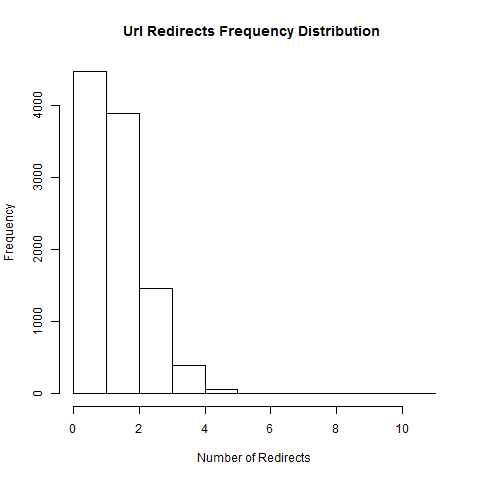
\includegraphics[scale=0.60]{url-redirect-histogram.png}
        \caption{Number of Redirects}
        \label{Number of Redirects}
    \end{center}
\end{figure}

%\newpage
\subsubsection{url-redirect-histogram.R}
\lstinputlisting[language=R,breaklines = true,frame=single,caption={R program to plot histogram for the number of redirects encountered}, label=lst:q2R,captionpos=b,numbers=left,showspaces=false,showstringspaces=false,basicstyle=\footnotesize]{url-redirect-histogram.R}

\newpage
\begin{figure}[ht]    
    \begin{center}
        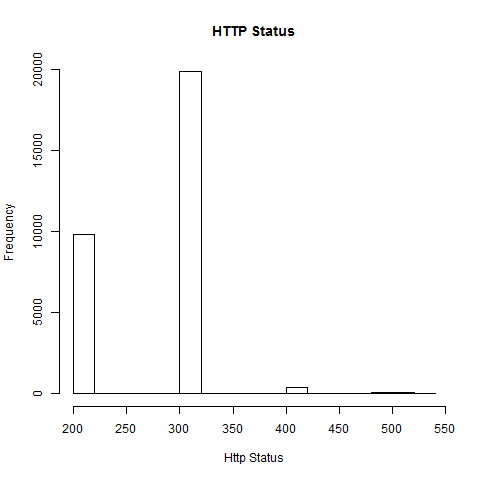
\includegraphics[scale=0.60]{http-statuses.png}
        \caption{HTTP statuses encountered}
        \label{HTTP statuses encountered}
    \end{center}
\end{figure}

%\newpage
\subsubsection{http-statuses.R}
\lstinputlisting[language=R,breaklines = true,frame=single,caption={R program to plot histogram for the HTTP statuses encountered}, label=lst:q2R,captionpos=b,numbers=left,showspaces=false,showstringspaces=false,basicstyle=\footnotesize]{http-statuses.R}




\section{Q2}
\label{part2}
\begin{enumerate}

\item Collection1: Extract all the unique terms and their frequency from the 10000 files*

\item Collection2: Extract all the unique terms and their frequency of the 10000 files* after running boilerpipe

\item Construct a table with the top 50 terms from each collection. 
	- Find a common stop word list.  How many of the 50 terms are on that stop word list?

\item For both collections, construct a graph with the x-axis as word rank, and y-axis as word frequency.  
	- Do either follow a Zipf distribution? Support your answer.

\end{enumerate}

\subsection{Solution}
\begin{enumerate}

\item I wrote two python programs to extract the unique terms and their frequency and saved it in text file.

\item In the collection1 there are 12 terms and in collection2 there are 41 terms that are from the stop word list. The stop word list is at the end of this document. The tables for both the collections with top 50 terms are shown below:

	\begin{table}
		\caption{Collection1: Word Frequency Table}
			\begin{center}
				\begin{tabular}{ c | c | c }
					\hline
Rank & Word & Word Frequency \\ \hline
1 & div & 1170684 \\ \hline
2 & a & 538390 \\ \hline
3 & li & 324226 \\ \hline
4 & span & 307373 \\ \hline
5 & script & 159971 \\ \hline
6 & ul & 129377 \\ \hline
7 & span & 120620 \\ \hline
8 & px & 110074 \\ \hline
9 & lia & 107868 \\ \hline
10 & the & 103445 \\ \hline
11 & meta & 100232 \\ \hline
12 & width & 97620 \\ \hline
13 & var & 97257 \\ \hline
14 & td & 93394 \\ \hline
15 & to & 86910 \\ \hline
16 & tr & 86689 \\ \hline
17 & img & 76837 \\ \hline
18 & height & 74584 \\ \hline
19 & and & 74201 \\ \hline
20 & p & 66089 \\ \hline
21 & typetext & 59865 \\ \hline
22 & javascript & 59865 \\ \hline
23 & link & 56247 \\ \hline
24 & in & 55901 \\ \hline
25 & false & 55637 \\ \hline
26 & of & 54765 \\ \hline
27 & h & 54099 \\ \hline
28 & if & 52750 \\ \hline
29 & de & 49659 \\ \hline
30 & button & 42086 \\ \hline
31 & targetblank & 42050 \\ \hline
32 & function & 41691 \\ \hline
33 & class & 41129 \\ \hline
34 & i & 40408 \\ \hline
35 & for & 39959 \\ \hline
36 & option & 38933 \\ \hline
37 & typebutton & 38543 \\ \hline
38 & input & 37612 \\ \hline
39 & onclickreturn & 33841 \\ \hline
40 & alt & 32257 \\ \hline
41 & on & 31724 \\ \hline
42 & is & 29757 \\ \hline
43 & href & 29362 \\ \hline
44 & with & 28148 \\ \hline
45 & border & 28143 \\ \hline
46 & br & 27742 \\ \hline
47 & this & 27409 \\ \hline
48 & value & 25635 \\ \hline
49 & your & 25497 \\ \hline
50 & color & 25470 \\ \hline
				\end{tabular}
			\end{center}  
	\end{table}  
	
	\begin{table}
		\caption{Collection2: Word Frequency Table}
			\begin{center}
				\begin{tabular}{ c | c | c }
					\hline
Rank & Word & Word Frequency \\ \hline
1 & the & 41228 \\ \hline
2 & to & 27058 \\ \hline
3 & a & 23068 \\ \hline
4 & and & 21496 \\ \hline
5 & of & 17275 \\ \hline
6 & in & 14449 \\ \hline
7 & is & 11417 \\ \hline
8 & you & 10493 \\ \hline
9 & for & 8928 \\ \hline
10 & this & 8494 \\ \hline
11 & play & 8330 \\ \hline
12 & on & 7955 \\ \hline
13 & your & 7593 \\ \hline
14 & that & 7545 \\ \hline
15 & it & 7250 \\ \hline
16 & now & 6905 \\ \hline
17 & que & 6760 \\ \hline
18 & with & 6335 \\ \hline
19 & i & 5735 \\ \hline
20 & are & 5187 \\ \hline
21 & y & 5070 \\ \hline
22 & as & 4928 \\ \hline
23 & be & 4858 \\ \hline
24 & next & 4632 \\ \hline
25 & by & 4579 \\ \hline
26 & have & 4355 \\ \hline
27 & or & 4209 \\ \hline
28 & not & 4119 \\ \hline
29 & from & 3512 \\ \hline
30 & no & 3486 \\ \hline
31 & more & 3388 \\ \hline
32 & at & 3301 \\ \hline
33 & has & 3263 \\ \hline
34 & was & 3191 \\ \hline
35 & but & 3170 \\ \hline
36 & will & 3101 \\ \hline
37 & an & 3043 \\ \hline
38 & we & 2961 \\ \hline
39 & can & 2915 \\ \hline
40 & if & 2764 \\ \hline
41 & all & 2560 \\ \hline
42 & up & 2402 \\ \hline
43 & they & 2357 \\ \hline
44 & he & 2284 \\ \hline
45 & new & 2164 \\ \hline
46 & add & 2151 \\ \hline
47 & been & 2063 \\ \hline
48 & get & 2049 \\ \hline
49 & about & 2011 \\ \hline
50 & when & 1991 \\ \hline
				\end{tabular}
			\end{center}  
	\end{table}  
  
\end{enumerate}



\newpage

\subsection{Graphs}
\begin{figure}[ht]    
    \begin{center}
        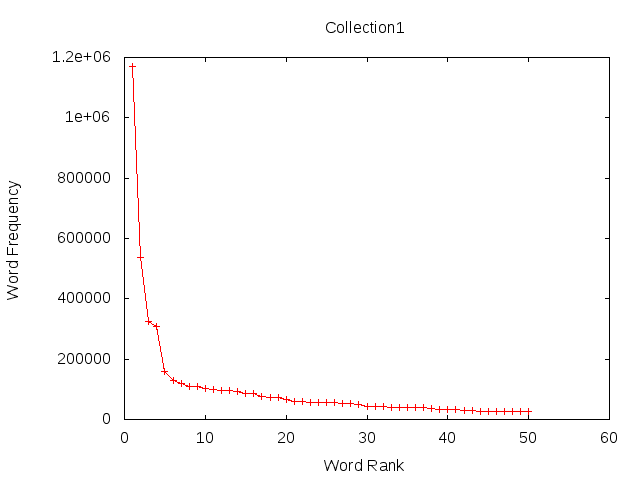
\includegraphics[scale=0.60]{plot_graph_c1.png}
        \caption{Graph for Collection1}        
    \end{center}
\end{figure}

\begin{figure}[ht]    
    \begin{center}
        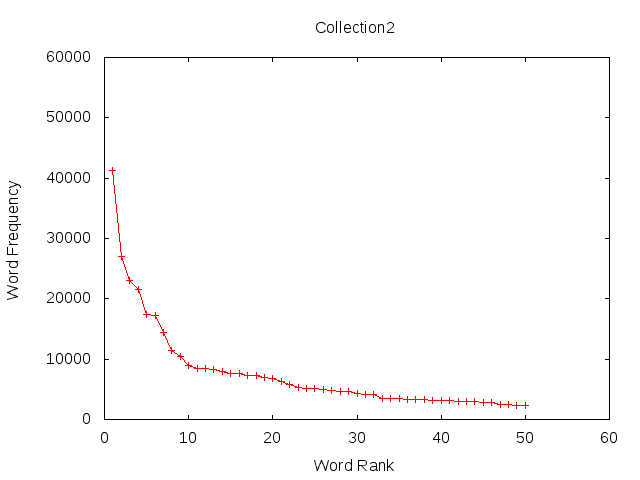
\includegraphics[scale=0.60]{plot_graph_c2.png}
        \caption{Graph for Collection2}        
    \end{center}
\end{figure}

Zipf law states that the frequency of any word is inversely proportional to its rank. In the above two graphs the value on Y axis decreases as the value on the X axis increases, which indicates that the frequency of the word is inversely proportional to its rank. Hence, both the collections follow Zipf distribution.

\newpage
\subsection{Code Listing}
\subsubsection{Collection 1: Python program to extract all the unique terms and their frequency from the 10,000 files generated by fetchWebpages.py}

\lstinputlisting[language=Python,breaklines = true,frame=single, label=lst:q1-1,captionpos=b,numbers=left,showspaces=false,showstringspaces=false,basicstyle=\footnotesize]{wordcount.py}
\newpage

\subsubsection{Collection 2: Python program to extract all the unique terms and their frequency of the 10,000 files after running boilerpipe}
\lstinputlisting[language=Python,breaklines = true,frame=single,label=lst:q1-1,captionpos=b,numbers=left,showspaces=false,showstringspaces=false,basicstyle=\footnotesize]{wordcountboilerpipe.py}
\newpage

\subsubsection{Collection 1: Ruby program using gnuplot to plot the word frequency distribution graph}
\lstinputlisting[language=Ruby,breaklines = true,frame=single,label=lst:q1-1,captionpos=b,numbers=left,showspaces=false,showstringspaces=false,basicstyle=\footnotesize]{plotgraphc1.rb}
\newpage

\subsubsection{Collection 2: Ruby program using gnuplot to plot the word frequency distribution graph}
\lstinputlisting[language=Ruby,breaklines = true,frame=single,label=lst:q1-1,captionpos=b,numbers=left,showspaces=false,showstringspaces=false,basicstyle=\footnotesize]{plotgraphc2.rb}

\newpage

\subsection{Stopword List}
\begingroup
\obeylines
\input{stopwords.txt}
\endgroup




\section{Q3}
\label{part3}
\begin{enumerate}

\item 3.1 Using 20 links that have TimeMaps
\subitem - With 20 or more mementos
\subitem - Have existed 2 years or more (i.e., Memento-Datetime of ``first memento" is April XX, 2013 or older)
\subitem - Note: select from Q1/Q2 links, else choose them by hand

\item 3.2 For each link, create a graph that shows Jaccard Distance, relative to the first memento, through time

\subitem x-axis: continuous time, y-axis: Jaccard Distance relative to the first memento



\end{enumerate}

\subsection{Solution}
\begin{enumerate}

\item I hand picked 20 timemaps from Q2.

\item I wrote a python program to process the timemaps, get the memento URIs, download the boilerpipe representation.

\item Next, I included the code for calculation of jacard distance of all other mementos relative to the first memento.

\item Following are few graphs that shows Jaccard Distance relative to the first memento, through time:


\newpage
\subsubsection{Graphs}
\begin{figure}[ht]    
    \begin{center}
        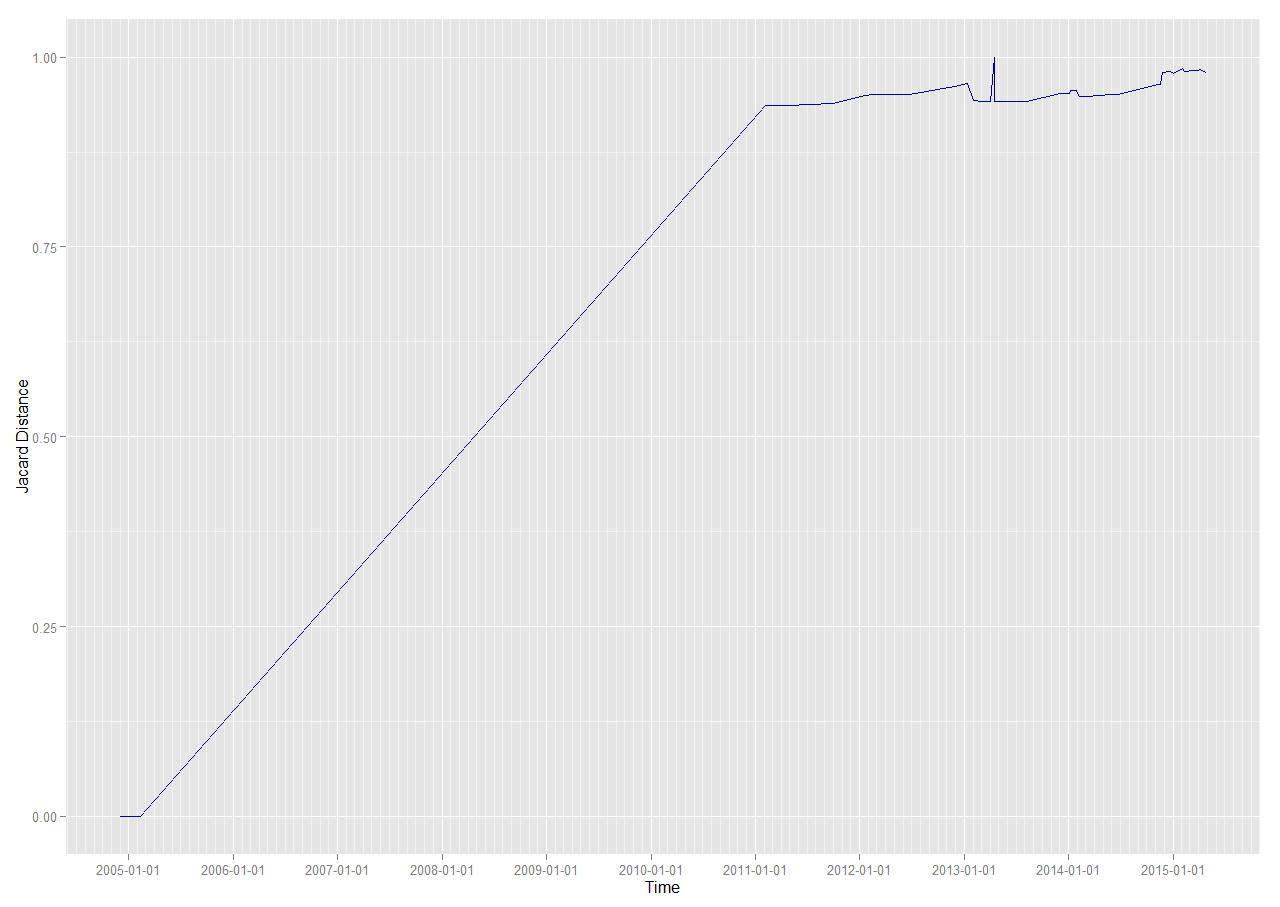
\includegraphics[scale=0.40]{graphs/3_j1.png}
        \caption{Memento 1}
    \end{center}
\end{figure}

\newpage
\begin{figure}[ht]    
    \begin{center}
        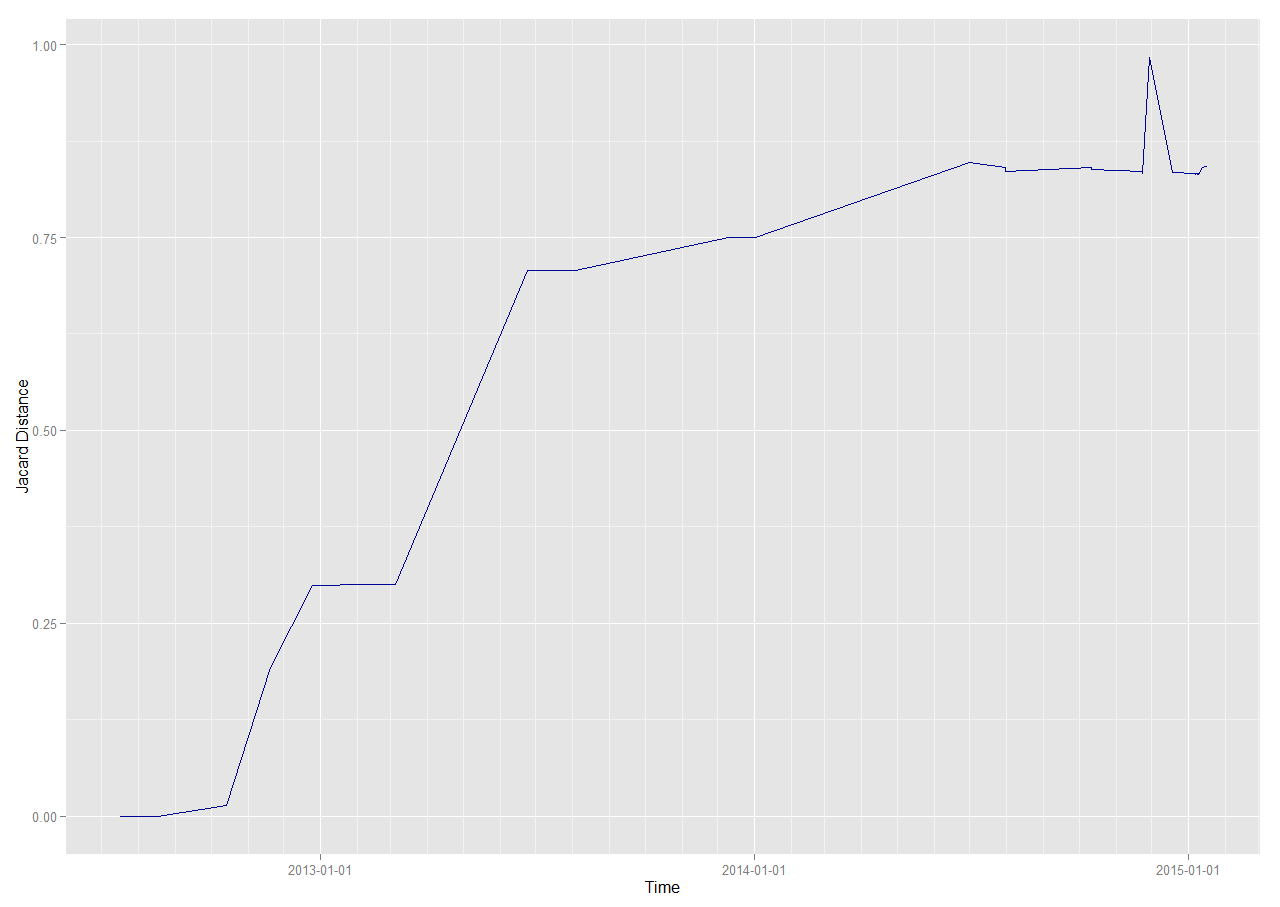
\includegraphics[scale=0.40]{graphs/3_j5.png}
        \caption{Memento 2}
    \end{center}
\end{figure}

\newpage
\begin{figure}[ht]    
    \begin{center}
        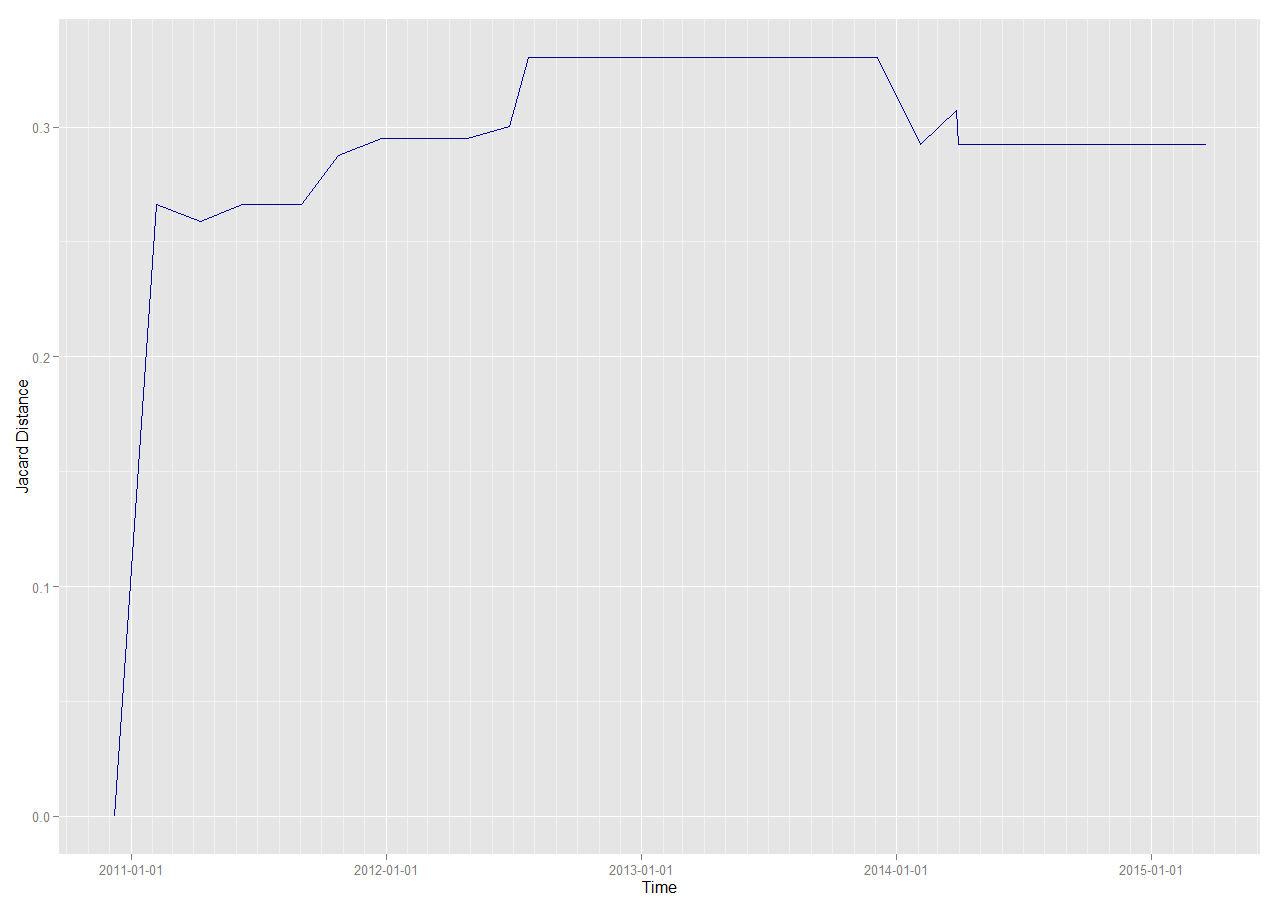
\includegraphics[scale=0.40]{graphs/3_j6.png}
        \caption{Memento 3}
    \end{center}
\end{figure}

\newpage
\begin{figure}[ht]    
    \begin{center}
        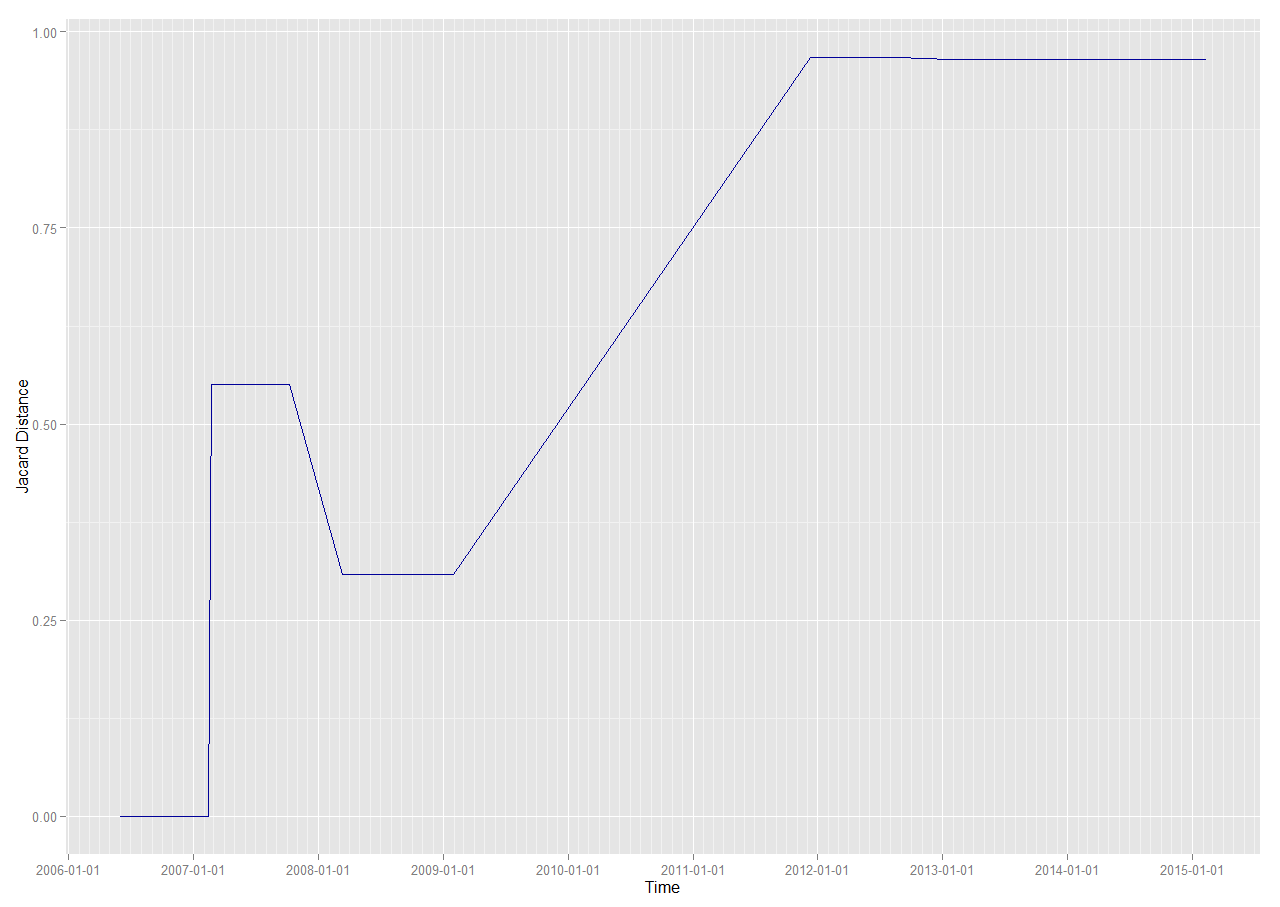
\includegraphics[scale=0.40]{graphs/3_j7.png}
        \caption{Memento 4}
    \end{center}
\end{figure}



\newpage
\subsection{Code Listing}
\subsubsection{Python program to using boilerpipe library to extract just the text from HTML documents of the mementos for the selected 20 timemaps}
\lstinputlisting[language=Python,breaklines = true,frame=single, label=lst:q1-1,captionpos=b,numbers=left,showspaces=false,showstringspaces=false,basicstyle=\footnotesize]{src/3.fetchBoilerpipeForMementos.py}
\newpage

\subsubsection{R code to plot CDF}
\lstinputlisting[language=Python,breaklines = true,frame=single, label=lst:q1-1,captionpos=b,numbers=left,showspaces=false,showstringspaces=false,basicstyle=\footnotesize]{src/3.r}

\end{enumerate}


\section{Q4}
\label{part4}
\begin{enumerate}

\item 3.1 Choose a news-related event

\item 3.2 Use twarc.py to collect 1000 tweets, every day for 5 different days
\subitem - See: \url{https://github.com/edsu/twarc}

\item 3.3 For each day:
\subitem - Create a wall
\subitem - Build a tag/word cloud for each day
\subitem - Create a map using GeoJSON and Github
\subsubitem - See: \url{https://help.github.com/articles/mapping-geojson-files-on-github/}

\item 3.4 Discuss in detail lessons learned, experiences, etc.

\end{enumerate}



\subsection{Solution}
\begin{enumerate}

\item I wrote a python program using `Twarc' library to collect daily 1000 tweets.
\item The news-related event that I chose was ``Nepal Earthquake".
\item Once I was done collecting the tweets, I used different tools in the Twarc package to get the wall, word cloud and geojson from these saved tweets.
\item Wall is a HTML document displaying the tweets with user handle, Tweet text, displays URLs if any, date time of the Tweet and displays the number of retweets.
\item Word Cloud is a HTML document which displays the cloud of most frequently used words in the list of tweets and displays these words as an image beautifully.
\item GeoJSON tool gives the locations from where the Tweet originated. It can give the location only if the Tweet has location information. Using this location information, github.com plots these on map.
\item Following are the screenshots of walls, word clouds and geojsons for 5 different days.

\newpage
\subsubsection{Walls}
\begin{figure}[ht]    
    \begin{center}
        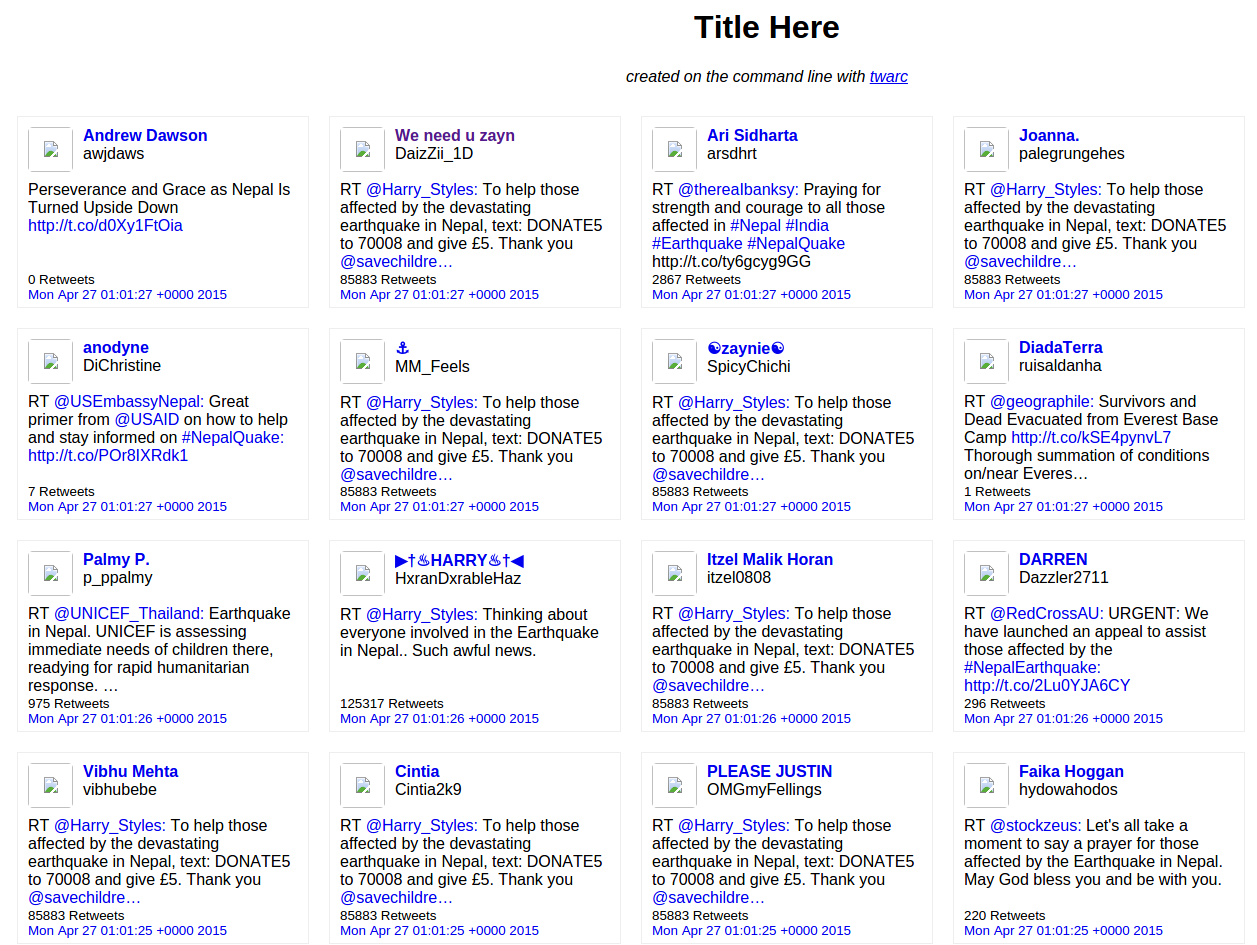
\includegraphics[scale=0.40]{graphs/wall1.png}
        \caption{Wall 1}
    \end{center}
\end{figure}

\newpage
\begin{figure}[ht]    
    \begin{center}
        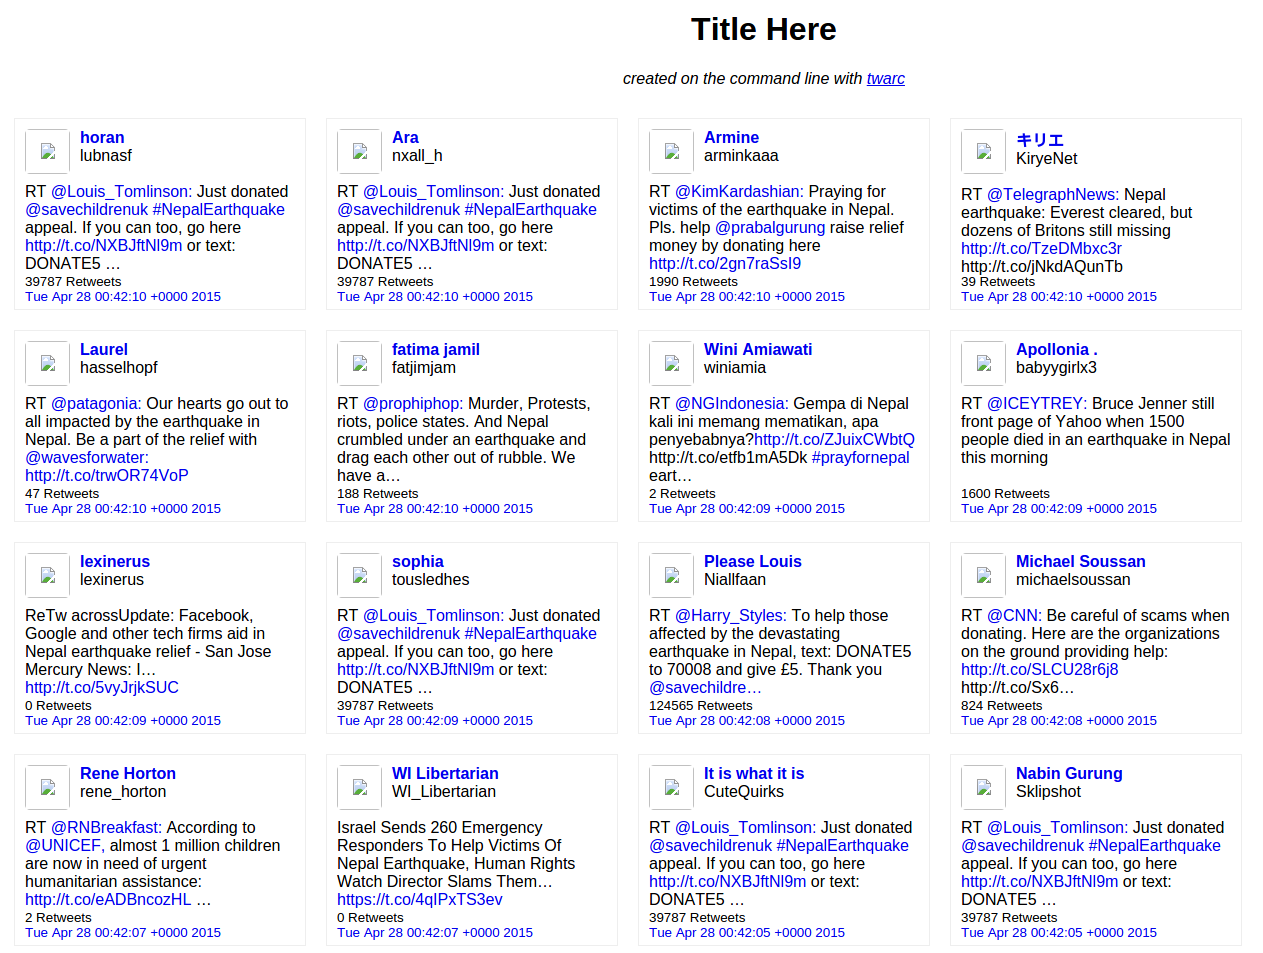
\includegraphics[scale=0.40]{graphs/wall2.png}
        \caption{Wall 2}
    \end{center}
\end{figure}

\newpage
\begin{figure}[ht]    
    \begin{center}
        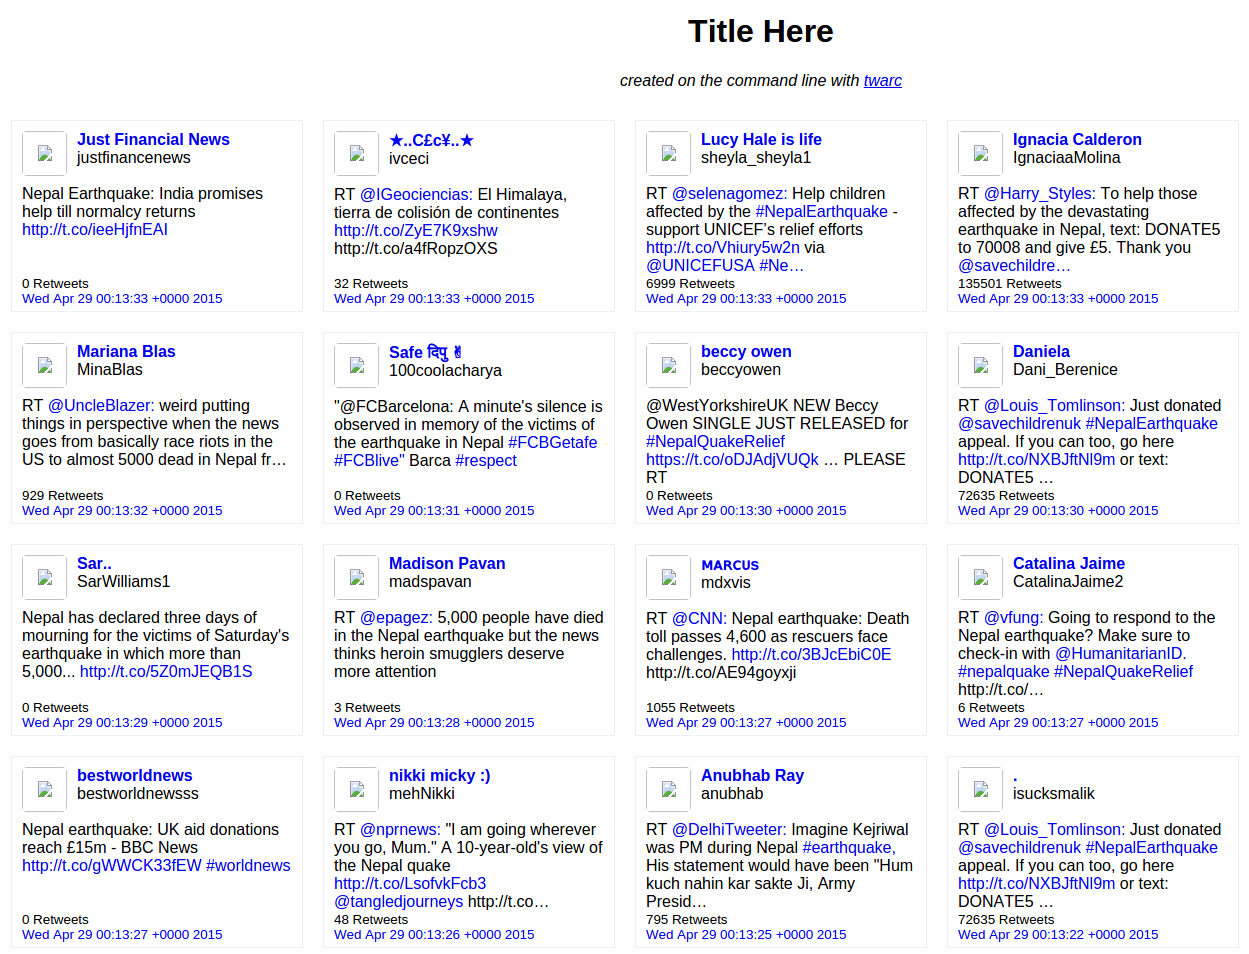
\includegraphics[scale=0.40]{graphs/wall3.png}
        \caption{Wall 3}
    \end{center}
\end{figure}

\newpage
\begin{figure}[ht]    
    \begin{center}
        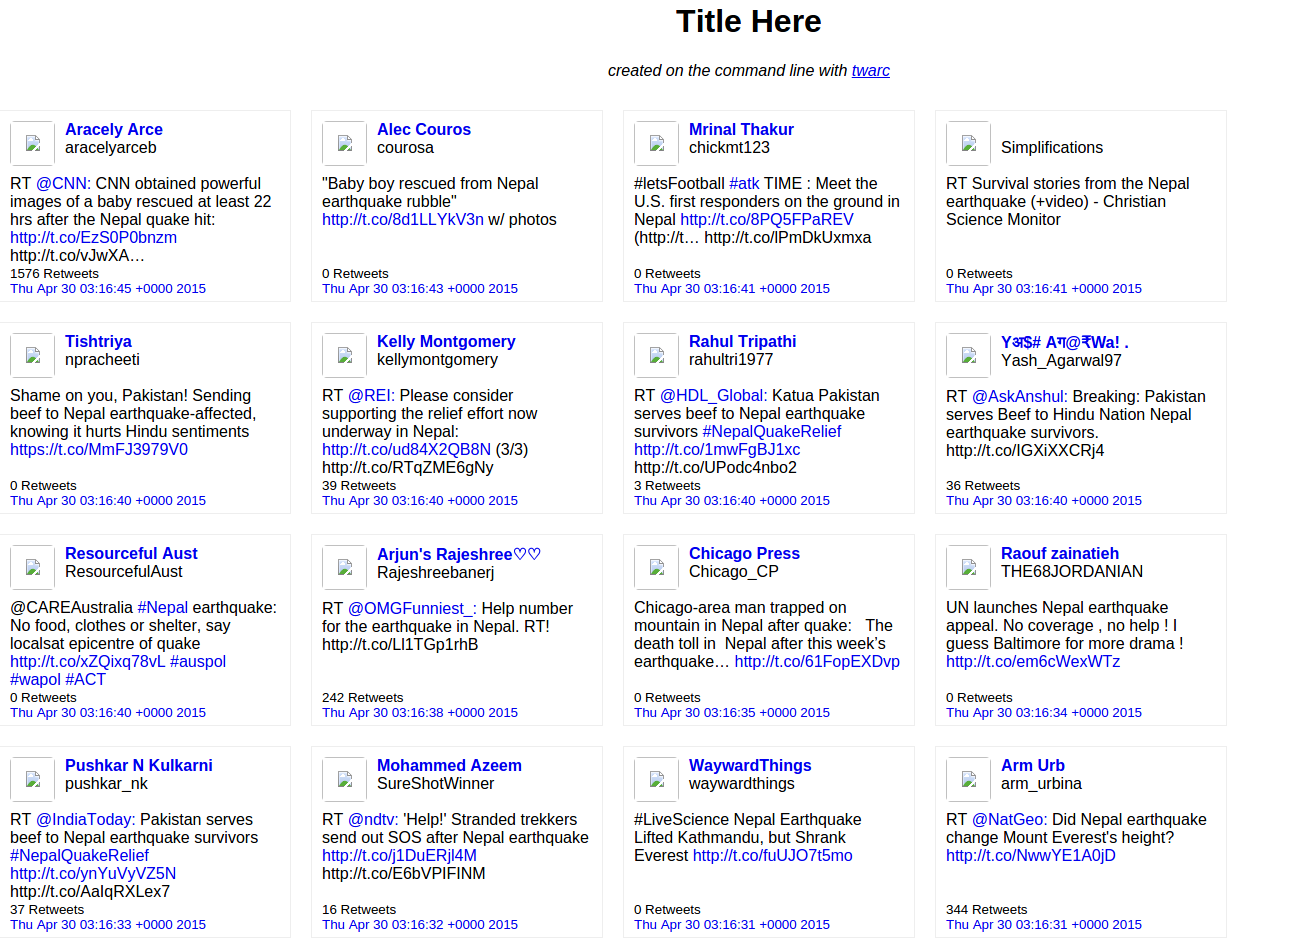
\includegraphics[scale=0.40]{graphs/wall4.png}
        \caption{Wall 4}
    \end{center}
\end{figure}

\newpage
\begin{figure}[ht]    
    \begin{center}
        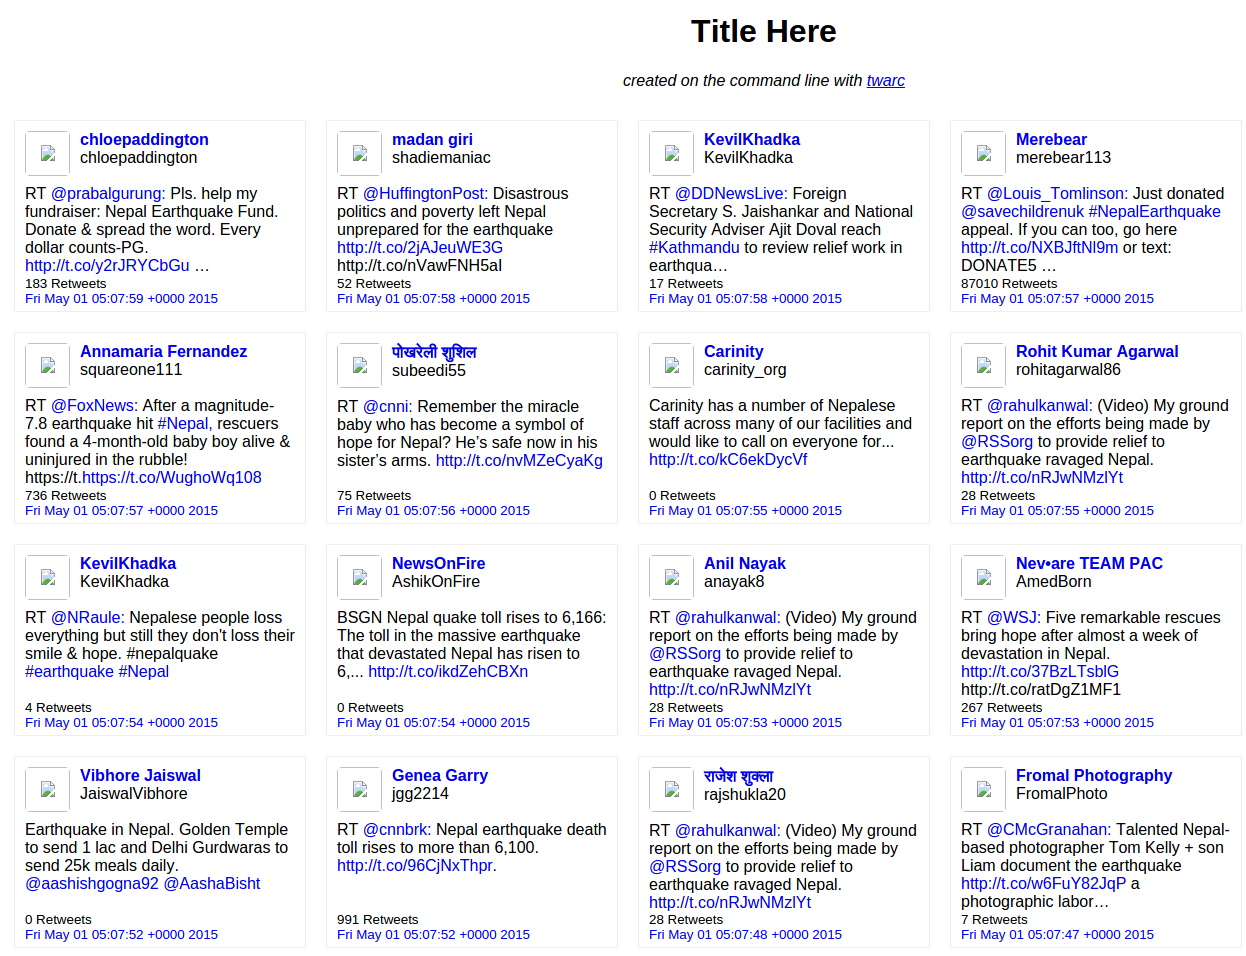
\includegraphics[scale=0.40]{graphs/wall5.png}
        \caption{Wall 5}
    \end{center}
\end{figure}

\newpage
\subsubsection{Word Clouds}
\begin{figure}[ht]    
    \begin{center}
        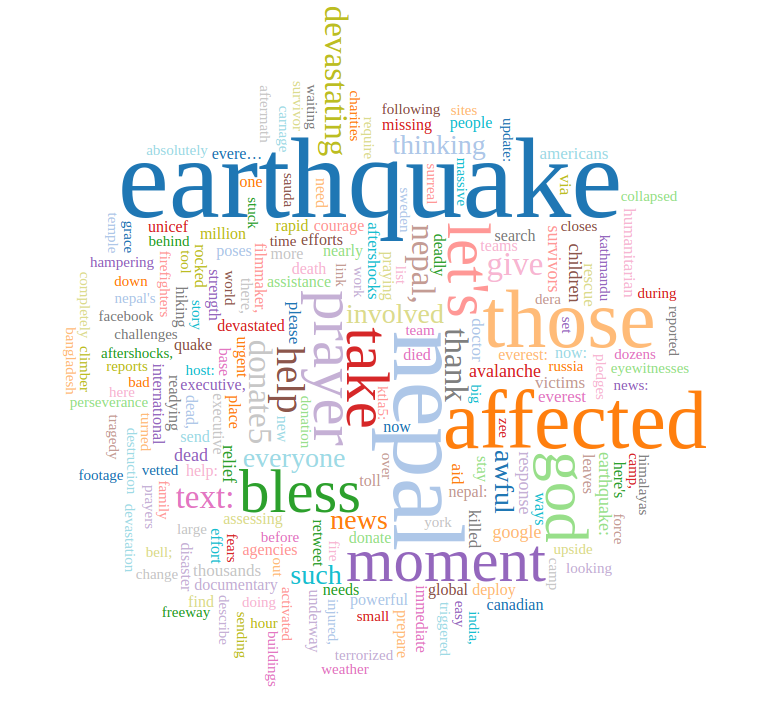
\includegraphics[scale=0.40]{graphs/wc1.png}
        \caption{Word Cloud 1}
    \end{center}
\end{figure}

\newpage
\begin{figure}[ht]    
    \begin{center}
        
\includegraphics[scale=0.40]{graphs/wc2.png}
        \caption{Word Cloud 2}
    \end{center}
\end{figure}

\newpage
\begin{figure}[ht]    
    \begin{center}
        
\includegraphics[scale=0.40]{graphs/wc3.png}
        \caption{Word Cloud 3}
    \end{center}
\end{figure}

\newpage
\begin{figure}[ht]    
    \begin{center}
        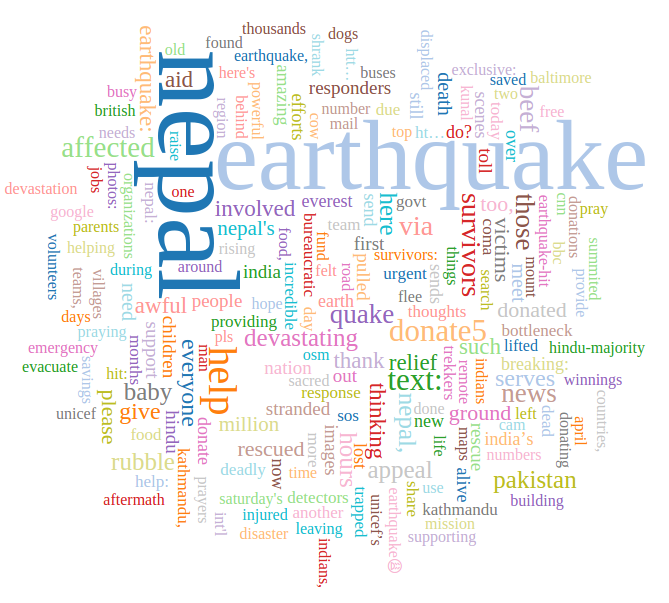
\includegraphics[scale=0.40]{graphs/wc4.png}
        \caption{Word Cloud 4}
    \end{center}
\end{figure}

\newpage
\begin{figure}[ht]    
    \begin{center}
        
\includegraphics[scale=0.40]{graphs/wc5.png}
        \caption{Word Cloud 5}
    \end{center}
\end{figure}

\newpage
\newpage
\newpage
\subsubsection{GeoJSONs}
\begin{figure}[ht]    
    \begin{center}
        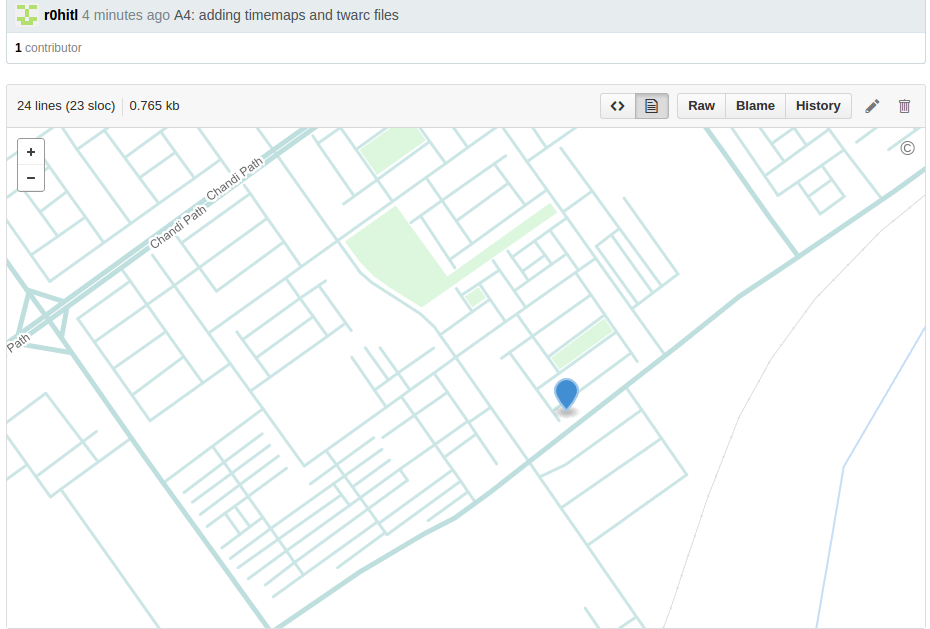
\includegraphics[scale=0.40]{graphs/gj1.png}
        \caption{GeoJSON 1}
    \end{center}
\end{figure}

\newpage
\begin{figure}[ht]    
    \begin{center}
        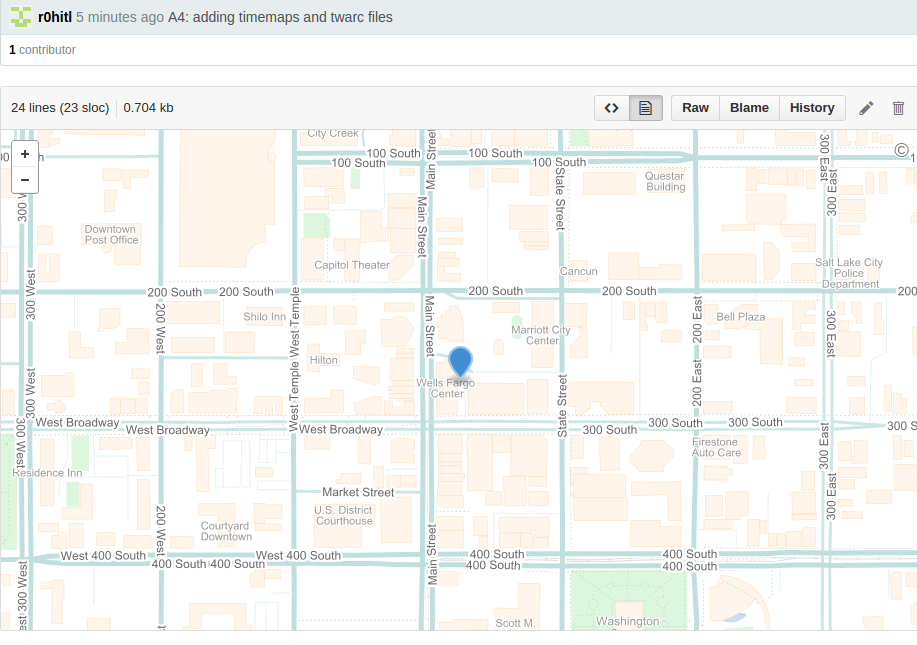
\includegraphics[scale=0.40]{graphs/gj2.png}
        \caption{GeoJSON 2}
    \end{center}
\end{figure}

\newpage
\begin{figure}[ht]    
    \begin{center}
        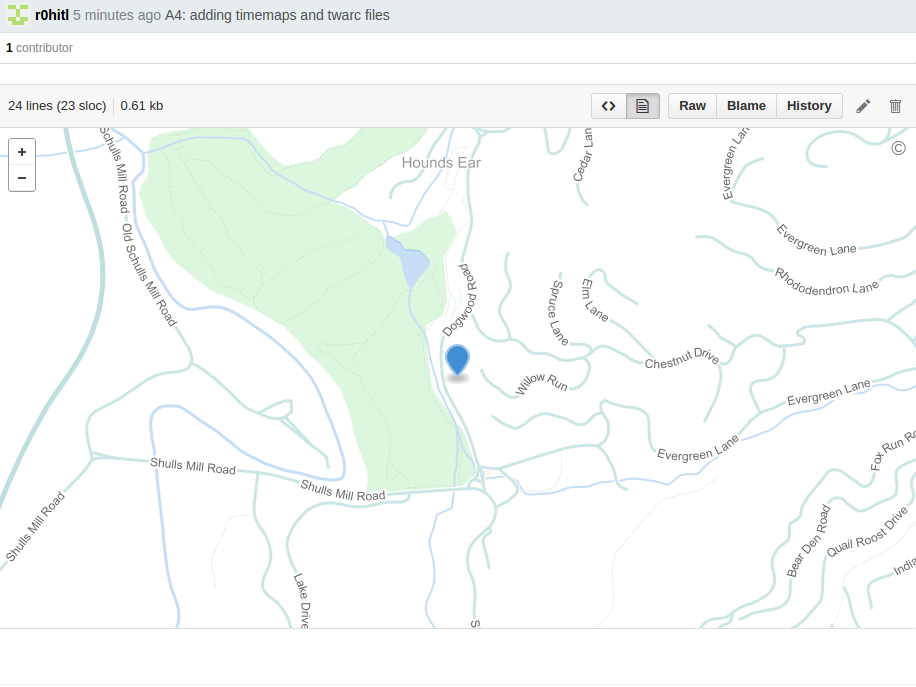
\includegraphics[scale=0.40]{graphs/gj3.png}
        \caption{GeoJSON 3}
    \end{center}
\end{figure}

\newpage
\begin{figure}[ht]    
    \begin{center}
        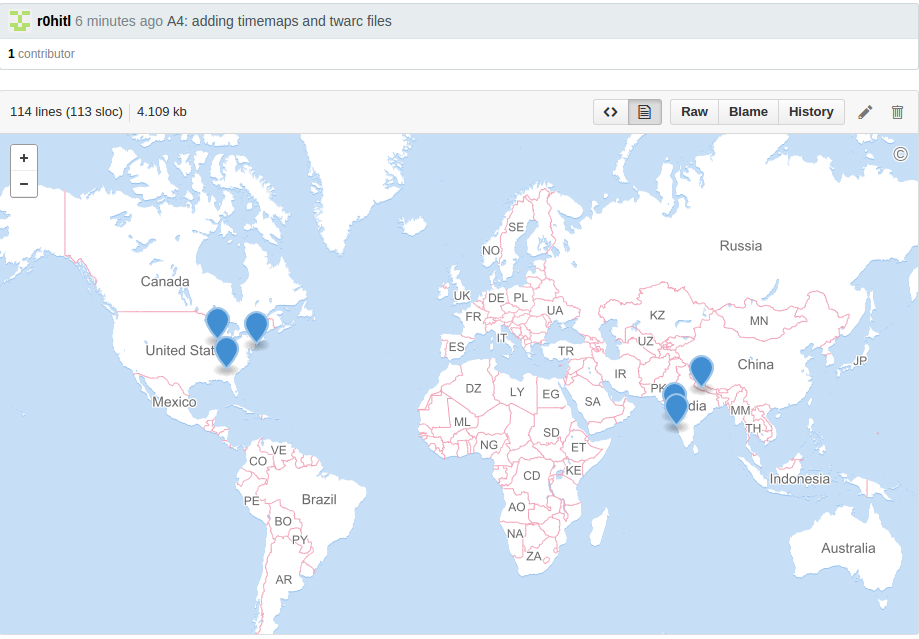
\includegraphics[scale=0.40]{graphs/gj4.png}
        \caption{GeoJSON 4}
    \end{center}
\end{figure}

\newpage
\begin{figure}[ht]    
    \begin{center}
        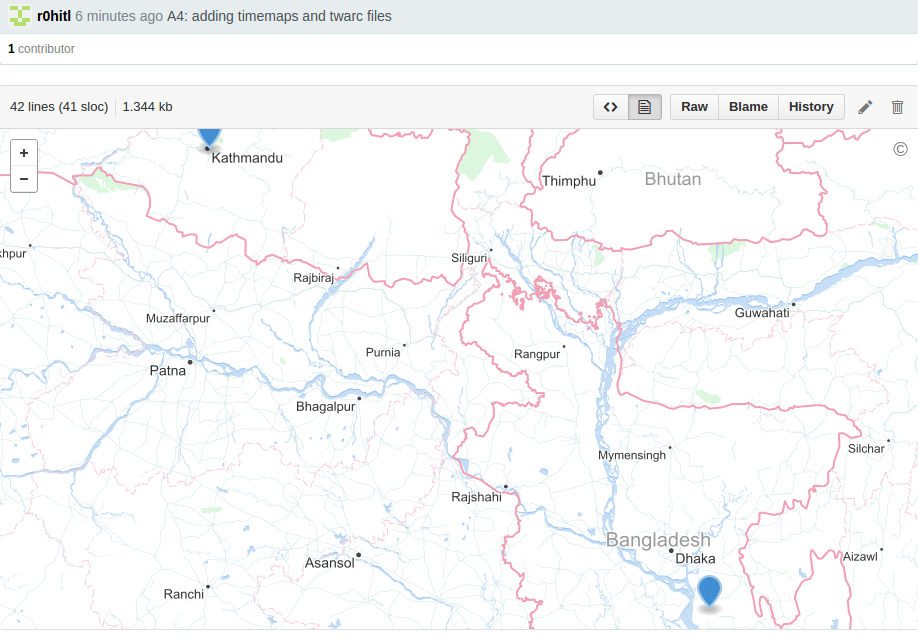
\includegraphics[scale=0.40]{graphs/gj5.png}
        \caption{GeoJSON 5}
    \end{center}
\end{figure}

\newpage
\subsection{Code Listing}
\subsubsection{Python program to fetch to fetch tweets using `twarc' library}
\lstinputlisting[language=Python,breaklines = true,frame=single, label=lst:q1-1,captionpos=b,numbers=left,showspaces=false,showstringspaces=false,basicstyle=\footnotesize]{src/4.tweetFetcherNepal.py}
\newpage

\end{enumerate}

%\bibliographystyle{plain}
%\bibliography{reference}
%\nocite{*}

\end{document}

